\chapter{Dasar Teori}
\label{chap:dasarteori}

Pada bab ini akan dijelaskan dasar-dasar teori mengenai arti baptis, pengertian calon baptis, cara menentukan nama baptis, sistem pendukung keputusan (SPK), Simple Additive Weighting (SAW), PHP, MySQL, dan bootstrap.

\section{Arti Baptis}
\label{sec:artibaptis}

Dalam agama Katolik, arti baptis merupakan sebuah sakramen yang berarti upacara suci \cite{sbaptis}. Baptis bukan hanya sekedar upacara belaka. Baptis merupakan awal dari usaha sepanjang hidup untuk berubah, agar dapat bersatu dengan Yesus dan menjadi lebih baik lagi dalam hal apapun. Tujuan dari baptis sendiri akhirnya adalah kita akan berbagi hidup dan kuasa dengan-Nya di dunia dan kelak selama-lamanya di surga. Sakramen baptis bagi umat Katolik menjelaskan bahwa:
\begin{enumerate}
	\item Allah menyelamatkan umat-Nya dengan cara ``Aku di dalam dia dan ia di dalam Aku'' (Yoh 6:56).
	\item Umat-Nya memaklumkan ``Ya, saya mau ``dimasuki'' Tuhan dan ``dimasukkan'' dalam Tuhan, sehingga Citra Allah dipulihkan'' (Yoh 15:5). ``Silahkan menggarap aku'', saya mau menyediakan kerjasama yang baik dengan Tuhan. 
\end{enumerate}

	Dalam sakramen baptis, air dituangkan atas kita. Kita secara perlahan dilebur menjadi satu dalam Kristus, namun kita tidak kehilangan identitas pribadi kita. Kita mempersatukan hidup kita dengan hidup-Nya. Tidak hanya bersatu dengan diri-Nya, tetapi juga menjadi bagian dari-Nya dan Ia juga menjadi bagian dari kita. Pembaptisan hanyalah merupakan awal dari suatu proses hidup untuk bersatu dengan Yesus. Kita tidak hanya bersatu secara fisik, tetapi juga bersatu secara mental dan spiritual. Gereja Katolik mengimani 3 makna air, yaitu:
	
	\begin{enumerate}
		\item Memberi hidup
		\item Membersihkan
		\item Memusnahkan dosa dan kejahatan
	\end{enumerate} 
	
	Yang terpenting dalam pembaptisan adalah membaptis dengan air yang suci atau air bersih, yang bergerak dinamis. Yang dimaksud dinamis adalah mengalir. Air yang mengalir tersebut biasa disebut sebagai ``air hidup''. Mereka juga membutuhkan seorang saksi dalam upacara Sakramen Baptis ini. Sebagai seorang Katolik yang utuh, maka seorang Katolik haruslah dibaptis. Syarat umum dalam Sakramen pembaptisan adalah setidaknya kehidupan calon baptis sudah meniru Tuhan Yesus dan juga ingin bersatu dengan diri-Nya. Seperti dalam Sabda Bahagia (Mat 5:3-12) yang diringkas menjadi Tiga Nasihat Injil adalah:
	
	\begin{itemize}
		\item Berjiwa miskin
		
		Nasihat yang pertama adalah berjiwa miskin. Kemiskinan menyebabkan seseorang merasa menderita, tetapi tidak semua orang yang miskin mendatangkan perasaan itu. Dengan cara menjalani hidup miskin, kita dapat merasa memiliki kekayaan jiwa untuk mendekatkan diri pada Tuhan. Hidupnya bergantung hanya pada Allah bukan pada harta.
		\item Taat
		
		Nasihat yang kedua adalah taat. Kita sebagai manusia mempunyai ``Tuan'' yaitu Allah. kita harus selalu menuruti perintah-Nya dan menjauhi larangan-Nya.
		\item Hidup suci 
		
		Nasihat yang ketiga adalah hidup suci. Hidup suci adalah benar-benar bersih dari dunia gemerlap malam hari (dugem), tidak mengejar kenikmatan diri, serta seutuhnya hidup untuk Tuhan dan sesama.
	\end{itemize}
	
	Seseorang tidak harus dibaptis ketika orang tersebut masih bayi, tetapi ada juga yang dibaptis ketika sudah dewasa. Pembaptisan yang dilakukan pada saat dewasa harus melalui beberapa persyaratan. Selain orang dewasa dan bayi yang harus dibaptis adalah:
	
	\begin{itemize}
		%\item Bayi
		
		%Pada bayi harus dibaptis sesegera mungkin sekitar 2-3 bulan setelah kelahirannya. Syarat mengikuti sakramen baptis untuk bayi adalah orang tuanya harus beragama Katolik dan menanam benih, agar tumbuh jadi pohon besar dan berbuah lebat, serta memiliki tanah yang subur.
		%\item Orang dewasa
	
		%Tidak hanya pada bayi, orang dewasa juga terdapat berbagai persyaratan untuk mengikuti Sakramen Pembaptisan. Syarat mengikuti Sakramen Baptis pada orang dewasa atau orang yang baru masuk katolik adalah:
		
		%\begin{itemize}
		%	\item Mengikuti pelajaran agama minimal 12 bulan
		%	\item Pengetahuan agama Katolik yang cukup
		%	\item Beriman
		%	\item Hidupnya meniru Tuhan Yesus
		%	\item Kehidupan gereja dan sosialisasi diri sudah baik
		%\end{itemize}
		\item  Orang beragama Katolik yang bersekolah di sekolah Katolik
		
		Bersekolah di sekolah Katolik dan orang tersebut beragama Katolik, tetapi belum dibaptis dan ingin dibaptis harus memenuhi beberapa syarat. Syarat untuk mengikuti sakramen baptisnya adalah cukup dengan mengikuti pelajaran agama minimal 7 bulan.
		
		\item Calon pengantin
		
		Persyaratan pada calon pengantin berbeda dengan orang dewasa. Syarat untuk mengikuti Sakramen Baptis untuk calon pengantin adalah cukup dengan mengikuti pelajaran tidak kurang dari 7 bulan.
		\item Orang yang sudah tua (60 tahun ke atas)
		
		Adapun orang yang sudah tua atau manula yang belum menjadi Katolik dan ingin menjadi Katolik. Syarat mengikuti sakramen baptis untuk orang yang sudah tua atau manula adalah sebagai berikut:
		
		\begin{itemize}
			\item Jika orang tersebut sudah pikun, dapat dibaptis dengan persiapan yang sangat pendek.
			\item Jika orang tersebut belum pikun harus menjalani beberapa persiapan secukupnya, seperti hafal doa-doa, pengetahuan agama yang cukup dan mengikuti kegiatan.
		\end{itemize}
		
		\item Orang gila
		
		Adapun sakramen baptis untuk orang gila.Jika orang gila tersebut, pada waktu tidak gilanya pernah menyatakan ingin mengikut Tuhan atau pernah ke gereja, maka akan dibaptis. Jika orang tersebut tidak pernah menyatakannya, maka tidak akan dibaptis.
		\item Dalam bahaya maut
		
		Dalam bahaya maut, siapapun orangnya dapat segera dibaptis dengan syarat hati orang tersebut suci dan penuh pertobatan, serta orang tersebut ingin beragama Katolik.
		
	\end{itemize} 
	Menurut Pastor A. Bogaarts, OSC sebagai Pastor Paroki di Gereja St. Laurentius, arti atau makna baptis sendiri untuk agama Katolik adalah suatu lambang lahiriah di mana diungkapkan, bahwa untuk menjadi anggota gereja Katolik yang secara resmi adalah diangkat menjadi anak Allah.
	
\section{Nama Baptis}
\label{sec:namabaptis1}
	
	Nama baptis mengingatkan orang yang dibaptis, bahwa ia tergabung dengan Kristus sebagai bagian dari diri-Nya dan ia didorong untuk hidup sesuai dengan panggilannya sebagai anak angkat Allah. Ia didorong sebagaimana yang ditunjukkan oleh teladan orang kudus, yang namanya diambil oleh ia melalui pembaptisan itu. Orang Katolik tidak diharuskan mempunyai nama baptis, tetapi boleh juga mempunyai nama baptis di bagian depan namanya.
	
	Pemakaian nama orang kudus atau santo-santa sebagai nama baptis sangatlah bermakna, baik, dan dianjurkan oleh Gereja. Gereja menganjurkan adanya nama baptis pada bagian depan nama calon baptis, dengan berbagai alasan tertentu, yaitu:
	
	\begin{itemize}
		\item Pemberian nama santo-santa pada saat pembaptisan adalah dengan maksud bahwa manusia ``lahir'' kembali sebagai manusia baru.
		\item Pemberian nama santo-santa mengingatkan akan adanya persekutuan orang kudus.
		\item Nama santo-santa yang kita ambil sebagai nama baptis dapat dijadikan sebagai santo-santa pelindung, dapat menjadi teladan, sehingga dapat meniru contoh kehidupan santo-santa tersebut dan kita dapat mengamalkan cinta kasih agar kita semakin mendekati Kristus.
	\end{itemize}
	
	
	Dalam memilih sebuah nama baptis yang cocok tidaklah sembarangan. Nama baptis benar-benar dipilih untuk menjadi teladan kita dan semakin dekat dengan Kristus. Dalam memilih nama baptis tidaklah hanya memilih berdasarkan namanya yang sesuai, bagus dan lain sebagainya. Melainkan nama baptis dipilih berdasarkan kriteria arti, lambang, tanggal pesta, ataupun cerita kehidupannya, agar kita sebagai calon baptis dapat mengerti, meneladani, dan dapat mengikuti atau meniru cerita kehidupannya (Lampiran \ref{fig:namabaptis1}, \ref{fig:namabaptis2}).
	
	Pada umumnya nama baptis mempunyai cerita kehidupan, lambang, arti, dan tanggal pesta santo-santa tersebut. Ada yang lengkap, ada juga yang tidak lengkap. Pada Lampiran \ref{fig:namabaptis1}, terdapat nama ``Agata''. Pada nama tersebut terdapat cerita kehidupan dari Agata, arti (A), lambang (L), dan tanggal pesta santo-santa (P) tersebut. Sedangkan pada Lampiran \ref{fig:namabaptis2}, terdapat nama ``Agatangelus'', yang pada nama tersebut hanya mengandung cerita kehidupan, arti (A), dan tanggal pesta santo-santa (P).
	
	Arti dan cerita kehidupan pada nama santo-santa sangat penting bagi calon baptis. Calon baptis yang memilihnya dapat mengikuti teladan santo-santa tersebut. Lambang yang dimiliki santo-santa juga dapat menjadi sebuah simbol. Tanggal pesta santo-santa pada nama santo-santa dapat dijadikan sebagai acuan jika orang tersebut ingin memilih nama baptis berdasarkan tanggal lahir ataupun tanggal pembaptisan mereka.
	
	Kriteria yang terdapat pada nama baptis tersebut, hanyalah untuk mempermudah kita dalam memilih nama baptis yang kita pilih. Nama baptis yang memiliki kriteria lengkap akan lebih mudah dalam mempertimbangkan nama tersebut tepat atau tidak untuk kita. Selain dapat mempermudah dalam memilih nama baptis, kita juga dapat mengerti dan mengikuti teladan dari nama santo-santa yang dipilih oleh calon baptis tersebut.
	
\section{Calon Baptis}
\label{sec:articalonbaptis}
	
	Untuk menjadi bagian dalam agama Katolik, seseorang harus melalui tahap baptis yang disebut Sakramen Baptis atau Sakramen Pembaptisan. Pembaptisan membebaskan calon baptis dari dosa asal, serta semua dosa pribadi dan dari hukuman akibat dosa-dosa tersebut. Selain membebaskan dari dosa, pembaptisan membuat orang yang dibaptis itu mengambil bagian dalam kehidupan Tritunggal Allah melalui rahmat yang menguduskan. Rahmat yang menguduskan adalah sebuah rahmat pembenaran yang mempersatukan pribadi yang bersangkutan dengan Kristus dan Gereja. Pada proses pembaptisan membutuhkan seseorang yang siap dibaptis dan siap mengikuti Kristus, yaitu calon baptis.
	
	
	Calon baptis adalah orang yang ingin menjadi Katolik, mengikut Kristus, mengikuti teladan-Nya, menjadi bagian dari-Nya, dan ingin bersatu dengan Kristus. Selain diterima sebagai anggota baru pada agama Katolik, para calon baptis juga diajak masuk ke kehidupan yang baru, di mana Kristus menjadi panutan utamanya. 
		
	
	Pada agama Katolik terdapat 3 tahap inisiasi Katolik. Tahap inisiasi Katolik adalah tahap di mana para calon baptis dari yang masih belum menjadi Katolik (calon) sampai menjadi anggota baru di Katolik atau dapat diartikan sebagai penerimaan seseorang masuk ke dalam atau menjadi anggota kelompok tertentu. Tahap inisiasinya adalah \cite{cbaptis}:
	
	\begin{itemize}
		\item Masa pra-katekumenat/simpatisan menjadi katekumen
		
			Pada masa ini, calon baptis mengalami masa pemurnian. Masa pemurnian yang dimaksud adalah calon merasa murni dan dituntut dalam pertobatan dan iman.
		\item Masa katekumen menjadi calon baptis
		
		Pada masa ini, calon baptis mengalami masa pengembangan. Pengembangan tersebut melalui ajaran agama, seperti pembinaan iman di Gereja. Pembinaan iman dimaksudkan agar calon baptis dapat siap secara iman menjadi Katolik dan mengikut Kristus. Selain dibina dan mendapatkan pengajaran, calon baptis juga harus melakukan kewajiban berupa tugas. Tugas yang harus dilakukan oleh calon baptis adalah mencatat ringkasan khotbah pada saat pastor sedang melakukan khotbah dan juga mengumpulkan tanda tangan pastor yang khotbah pada waktu itu.
		\item Masa calon baptis menjadi baptisan baru
		
		Pada masa ini, calon baptis sudah benar-benar siap secara iman untuk mengikuti Kristus dan teladan-Nya. Calon baptis akan menjadi anggota gereja Katolik yang baru.
	\end{itemize}

%\section{Cara Pembaptisan}
%\label{sec:carabaptis}

	%Pada agama Katolik, Sakramen Baptis mempunyai cara tersendiri. Cara pembaptisan pada bayi (Gambar \ref{fig:baptis}) dan orang dewasa (Gambar \ref{fig:baptis1}) pada dasarnya sama, yaitu pastor ataupun diakon menuangkan air suci pada bagian dahi calon baptis atau menenggelamkan calon baptis dan mengucapkan ``Aku membaptis kamu dalam nama Bapa, Putra dan Roh Kudus'' (Matius 28:19), dengan menggunakan air yang mengalir yang telah diberkati, karena air percikan tidak cukup. Air percikan tidak cukup karena tidak dapat membasuh semua dahi kita, atau tidak membasuh semua tubuh kita.
	
	%Dalam wawancara yang telah dilakukan dengan Pastor A. Bogaarts, OSC, menurut beliau, ada beberapa kelemahan dan keuntungan ketika baptis pada waktu bayi. Kelemahannya adalah kurangnya mendapatkan pendalaman iman. Keuntungannya adalah telah mengikut Kristus dari sewaktu Bayi. Sedangkan jika baptis dewasa, yaitu benar-benar belajar. Yang dimaksud belajar adalah dengan cara mencari komunitas Katolik atau dapat membantu dia memilih Kristus sebagai Juru Selamat dan dapat lebih mendalami iman. Untuk orang dewasa yang ingin dibaptis, harus mengikuti pelajaran agama. Pelajaran agama tersebut juga memberikan tugas, seperti menulis khotbah Pastor, serta mengumpulkan tanda tangan Pastor yang khotbah pada waktu itu.
	
		%\begin{figure}[htbp]
		%\centering
		%	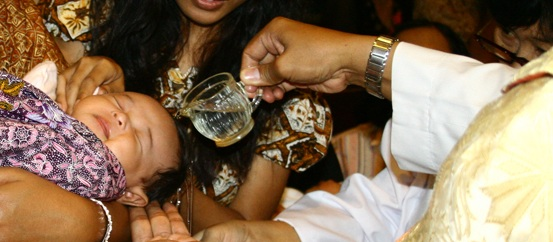
\includegraphics[scale=0.4]{Gambar/baptis.jpg}
		%\caption{Baptis Bayi}
		%\label{fig:baptis}
	%\end{figure}
	
	%\begin{figure}[ht]
	%	\centering
	%		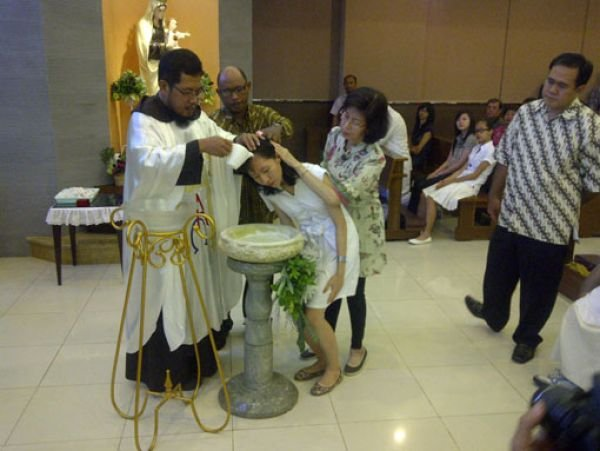
\includegraphics[scale=0.4]{Gambar/baptis1.jpg}
	%	\caption{Baptis Dewasa}
	%	\label{fig:baptis1}
	%\end{figure}
		
		
\section{Cara Menentukan Nama Baptis}
\label{sec:caramenentukannamabaptis}

Dalam menentukan nama baptis tidaklah mudah. Dibutuhkan pengetahuan akan nama-nama baptis Katolik. Menurut Pastor A. Bogaarts, OSC, dalam memilih atau menentukan nama Baptis tidak ada kriteria tertentu atau dapat dikatakan ``bebas memilih'', tetapi sebaiknya kita memilih orang kudus yang sekiranya dekat dengan bakat kita atau nama karena mirip atau memilih karena artinya. Selain itu tanggal lahir, tanggal pembaptisan, serta pesta nama baptis juga bisa dijadikan acuan dalam memilih nama baptis. 

%analisis
%Berdasarkan kuisioner yang telah disebarkan pada tanggal 7 Februari 2016 (Gambar \ref{fig:kuisioner1}), didapat data sebagai berikut:
%\begin{itemize}
	%\item Tanggal lahir sebanyak 6 orang
	%\item Tanggal Pembaptisan sebanyak 3 orang
	%\item Deskripsi Santo-Santa sebanyak 20 orang
	%\item Pesta Santo-Santa sebanyak 1 orang
	%\item Profesi Santo-Santa sebanyak 4 orang
	%\item Arti Nama Santo-Santa sebanyak 24 orang
	%\item Lambang dari Santo-Santa sebanyak 4 orang
	%\item Lain-lain sebanyak 5 orang
%\end{itemize}

%\begin{figure}[htbp]
	%	\centering
		%	\includegraphics[scale=0.4]{Gambar/capture.jpg}
		%\caption{Data Kuisioner Berdasarkan Kategori Pemilihan Nama Baptis}
		%\label{fig:kuisioner1}
	%\end{figure}
 \section{Sistem Pendukung Keputusan}
\label{sec:analisisspk}

Menurut Raymond McLeod (1998) dalam jurnal Teknik Informatika oleh Verina Valensia dan kawan-kawan bahwa SPK (Sistem Pendukung Keputusan) adalah sebuah sistem penghasil informasi spesifik yang ditujukan untuk memecahkan suatu masalah tertentu yang harus dipecahkan oleh manager pada berbagai tingkatan \cite{spk1}. Menurut Litle (1970), dalam jurnal Teknik Informatika oleh Verina Valensia dan kawan-kawan bahwa SPK adalah suatu sistem informasi berbasis komputer yang menghasilkan berbagai alternatif keputusan untuk membantu manajemen dalam menangani berbagai permasalahan yang terstruktur dengan menggunakan data dan model. 

Secara umum, SPK adalah sistem yang mampu memberikan kemampuan, baik kemampuan pemecahan masalah maupun kemampuan pengkomunikasian untuk masalah semi-terstruktur \cite{spk1}. Sedangkan secara khusus, SPK adalah sebuah sistem yang mendukung kerja seorang manager maupun sekelompok manager dalam memecahkan masalah semi-terstruktur. Pemecahan masalahnya adalah dengan cara memberikan informasi ataupun usulan untuk mendapatkan keputusan tertentu. Dapat ditarik kesimpulan, bahwa SPK atau yang biasa disebut DSS (\textit{Decision Support Systems}) adalah bagian dari sistem informasi berbasiskan komputer. SPK digunakan untuk mendukung pengambilan keputusan dalam suatu organisasi atau perusahaan ataupun seseorang. Menurut Moore and Chang, SPK dapat digambarkan sebagai sistem yang berkemampuan mendukung analisis \textit{ad hoc} data, pemodelan keputusan, berorientasi keputusan dan orientasi perencanaan masa depan. Kerangka dasar pengambilan keputusan manajerial dalam tipe keputusan dibagi menjadi  \cite{spk1}:	
	\begin{enumerate}
		\item Keputusan Terstruktur (\textit{structured decision}) \\
		Keputusan Terstruktur adalah sebuah keputusan yang berulang-ulang dan rutin, sehingga dapat diprogram. Keputusan terstruktur terjadi dan dilakukan terutama pada manajemen tingkat bawah. Contoh dari keputusan tipe ini adalah keputusan pemesanan barang, keputusan penagihan piutang dan lain sebagainya.
		\item Keputusan Tidak Terstruktur (\textit{unstructured decision})\\
		Keputusan Tidak Terstruktur adalah sebuah keputusan yang tidak terjadi berulang-ulang dan tidak selalu terjadi. Keputusan pada tipe ini terjadi dan dilakukan terutama pada manajemen tingkat atas. Informasi tidak mudah didapatkan, tidak mudah tersedia, dan biasanya berasal dari lingkungan luar. Contoh dari keputusan tipe ini adalah keputusan untuk bergabung dengan perusahaan lain.
		\item Keputusan Semi Terstruktur (\textit{semi-structured decision})\\
		Keputusan Semi Terstruktur adalah keputusan yang sebagian dapat diprogram, sebagian dapat berulang-ulang dan rutin, tetapi sebagian tidak terstruktur. Keputusan tipe ini bersifat rumit dan membutuhkan perhitungan serta analisis yang terperinci. Contoh dari keputusan tipe ini adalah keputusan alokasi dana promosi.
	\end{enumerate}
	
	SPK mempunyai beberapa tujuan dalam mendukung suatu keputusan dalam suatu organisasi atau perusahaan ataupun seseorang. Tujuan dari SPK adalah sebagai berikut:
	
	\begin{enumerate}
		\item Membantu menyelesaikan masalah semi-terstuktur
		\item Mendukung manajer dalam mengambil keputusan suatu masalah
		\item Meningkatkan efektifitas bukan efisiensi pengambilan keputusan
	\end{enumerate}

	Dalam sebuah SPK, terdapat \textit{Fuzzy Multiple Attribute Decision Making} (FMADM) yang adalah suatu metode yang digunakan untuk mencari alternatif optimal dari sejumlah alternatif dengan kriteria tertentu. Dalam FMADM, kita dapat menentukan nilai bobot untuk setiap atribut, yang kemudian dilanjutkan dengan proses perankingan yang akan menyeleksi alternatif yang sudah diberikan. Ada beberapa metode yang dapat digunakan untuk menyelesaikan masalah FMADM, antara lain:
	
	\begin{enumerate}
		\item \textit{Simple Additive Weighting Method} (SAW)
		\item \textit{Weighted Product} (WP)
		\item ELECTRE
		\item \textit{Technique for Order Preference by Similarity to Ideal Solution}(TOPSIS)
		\item \textit{Analytic Hierarchy Process}(AHP)
	\end{enumerate}
	
	
 %Salah satu metode yang akan dibahas pada topik ini adalah \textit{Simple Additive Weighting Method} (SAW). Metode ini sering dikenal dengan metode penjumlahan terbobot. Konsep dasar pada metode SAW adalah mencari penjumlahan terbobot dari rating kinerja pada setiap alternatif pada semua atribut. Metode ini berguna untuk pengambilan keputusan dalam suatu kasus, tetapi perhitungan dengan menggunakan metode SAW ini hanya yang menghasilkan nilai terbesar yang akan terpilih sebagai alternatif terbaik. Metode SAW ini lebih efisien karena waktu yang dibutuhkan dalam perhitungan lebih singkat. Metode ini membutuhkan proses normalisasi matriks keputusan ke suatu skala yang dapat diperbandingkan dengan semua rating alternatif yang ada.

	Ada berbagai macam masalah yang dialami oleh seseorang, perusahaan dan lain-lain dalam kehidupan sehari-hari. Masalah dapat dipecahkan atau dapat diselesaikan dengan baik jika sudah mengerti permasalahan utamanya seperti apa. Jika seseorang ataupun sebuah perusahaan telah mengetahui permasalahan mereka, maka mereka akan membuat sebuah keputusan. Keputusan yang dihasilkan merupakan sebuah keputusan yang terbaik bagi mereka. Adapun tahapannya dalam mengambil sebuah keputusan. SPK mempunyai tahapan proses pengambilan keputusan, diantaranya adalah sebagai berikut \cite{karakteristikspk}:
	\begin{itemize}
		\item Tahap Penelusuran
			
			Tahap ini merupakan proses penelusuran, pendeteksian dari lingkup problematika, serta proses pengenalan masalah. Data yang diperoleh diproses dan diuji dalam rangka mengidentifikasikan masalah.
		\item Tahap Perancangan
		
	Tahap ini merupakan proses menemukan, mengembangkan dan menganalisis tindakan yang mungkin dilakukan. Hal ini meliputi pemahaman terhadap masalah dan menguji solusi yang layak.
		\item Tahap Pemilihan
		
		Pada tahap ini dibuat suatu keputusan yang nyata dan diambil suatu komitmen untuk mengikuti suatu tindakan tertentu.
		\item Tahap Implementasi
		
		Pada tahap ini dibuat suatu solusi yang direkomendasikan dapat bekerja atau implementasi solusi yang diusulkan untuk suatu masalah.
		
	\end{itemize}
	
		Diperlukan tahapan-tahapan diatas karena sebuah masalah atau persoalan pasti mempunyai informasi yang harus dipertimbangkan untuk dipilih menjadi yang terbaik. Oleh karena itu, SPK berbasiskan komputer ini, dapat membantu memecahkan persoalan atau masalah-masalah yang sering dihadapi oleh perusahaan, organisasi ataupun seseorang dengan mengumpulkan data dan mengolahnya menjadi sebuah informasi.
		
		Selain mempunyai tahapan pada pemilihan alternatifnya, SPK juga mempunyai beberapa karakteristik. Karakteristik SPK adalah sebagai berikut \cite{karakteristikspk}:
		
		\begin{enumerate}
			\item Mendukung pengambilan keputusan untuk membahas masalah-masalah terstruktur, semi-terstruktur, dan tidak terstruktur.
			\item Output ditujukan bagi personil organisasi dalam semua tingkatan.
			\item Mendukung masing-masing fase pada proses pengambilan keputusan: penelusuran, perancangan, dan pemilihan.
			\item Adanya antar-muka (\textit{interface}) manusia atau mesin, di mana manusia tetap mengontrol proses pengambilan keputusan.
			\item Menggunakan model matematis dan statistik yang sesuai dengan pembahasan.
			\item Memiliki kemampuan dialog untuk memperoleh informasi sesuai dengan kebutuhan.
			\item Memiliki subsistem-subsistem yang terintegrasi sedemikian serupa, sehingga dapat berfungsi sebagai kesatuan sistem.
			\item Membutuhkan struktur data komprehensif yang dapat melayani kebutuhan informasi seluruh tingkatan manajemen. Data komprehensif adalah data yang memiliki sifat mampu menangkap atau menerima data dengan baik.
			\item Pendekatan \textit{easy to use}. Ciri suatu sistem pendukung keputusan yang efektif adalah kemudahannya untuk digunakan dan memungkinkan keleluasaan pemakai untuk memilih atau mengembangkan pendekatan-pendekatan baru dalam membahas masalah yang dihadapi.
			\item Kemampuan sistem untuk beradaptasi secara cepat, di mana pengambil keputusan dapat menghadapi masalah-masalah baru dan pada saat yang sama dapat menanganinya dengan cara mengadaptasikan sistem terhadap kondisi-kondisi perubahan yang terjadi.
		\end{enumerate}
		
		Dengan demikian, SPK sangatlah berguna dalam kehidupan sehari-hari. Dengan menggunakan SPK, kita dapat memecahkan suatu masalah dengan baik, karena adanya beberapa alternatif solusi yang baik. Alternatif solusi tersebut dapat kita pilih sesuai dengan yang mendekati atau yang sama dengan yang kita inginkan.
		
		
\section{Simple Additive Weighting (SAW)}
\label{sec:saw}
SPK mempunyai metode yang sangat banyak, salah satunya adalah metode SAW. Metode \textit{Simple Additive Weighting} (SAW) sering dikenal dengan metode penjumlahan terbobot. Konsep dasar pada metode SAW adalah mencari penjumlahan terbobot dari rating kinerja pada setiap alternatif pada semua atribut. Metode ini berguna untuk pengambilan keputusan dalam suatu kasus. Perhitungan dengan menggunakan metode SAW ini menghasilkan nilai dari nilai terbesar hingga nilai terkecil. Nilai terbesar yang akan terpilih sebagai alternatif terbaik, selebihnya merupakan nilai terbesar kedua, ketiga, dan seterusnya akan dijadikan sebagai alternatif lain. Metode SAW ini lebih efisien karena waktu yang dibutuhkan dalam perhitungan lebih singkat daripada dengan metode FMADM yang lain, seperti AHP, ELECTRE, dan metode FMADM lainnya. Metode ini membutuhkan proses normalisasi matriks keputusan ke suatu skala yang dapat diperbandingkan dengan semua rating alternatif yang ada. %Proses normalisasi adalah sebuah proses yang mengelompokkan data menjadi satu.

Pada metode SAW, terdapat proses normalisasi. Normalisasi adalah sebuah proses yang menormalisasikan matriks keputusan (X) ke suatu skala, yang dapat diperbandingkan dengan semua rating alternatif yang ada. Dengan kata lain, normalisasi adalah sebuah proses pengelompokkan data menjadi satu kategori dan diperbandingkan. Normalisasi dikelompokkan menjadi 2 atribut, yaitu atribut keuntungan (\textit{benefit}) dan atribut biaya (\textit{cost}). Perbedaan mendasar dari kedua atribut ini adalah dalam pemilihan kriteria. Jika seseorang memilih kriteria yang mengandung sebuah keuntungan, maka akan dilakukan proses normalisasi menggunakan atribut keuntungan, begitu juga sebaliknya. Pada kelompok kedua atribut tersebut dibutuhkan proses normalisasi dengan sebuah formula normalisasi.  Untuk melakukan normalisasi tersebut dibutuhkan sebuah formula sebagai berikut:

\[ r_{ij}  =
  \begin{cases}
    \frac{x_{ij}}{\stackrel{Max}{i} x_{ij}}      & \quad \text{jika } j \text{ adalah atribut keuntungan (\textit{benefit})}\\
		
		
  \frac{\stackrel{Min}{i} x_{ij}} {x_{ij}}     & \quad \text{jika } j \text{ adalah atribut biaya (\textit{cost})}\\
  \end{cases}
\]

%\begin{figure}[htbp]
	%	\centering
		%	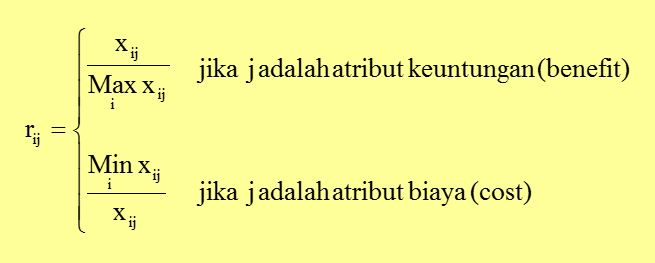
\includegraphics[scale=0.4]{Gambar/saw1.jpg}
		%\caption{Formula Normalisasi}
		%\label{fig:formulanormalisasi}
%	\end{figure}
	
	Keterangan:
	
	\begin{itemize}
		\item $r_{ij}$ = Nilai rating kinerja
		\item $x_{ij}$ = Nilai kinerja dari setiap rating
		\item $Max 	 x_{ij}$ = Nilai terbesar dari tiap kriteria
		\item $Min 	 x_{ij}$ = Nilai terkecil dari tiap kriteria
		\item $i$ = alternatif
		\item $j$ = kriteria
\end{itemize}
	
dengan $r_{ij}$ adalah rating kinerja ternormalisasi dari alternatif ($A_{i}$) pada atribut $C_{j}$; i= 1,2,...,m dan j= 1,2,...,n. Nilai preferensi untuk setiap alternatif diberikan sebagai berikut: 

\[
 V_{i} =\displaystyle\sum_{j=1}^{n} w_{j} r_{ij}
\]

Keterangan:
\begin{itemize}
	\item $V_{i}$ = Nilai akhir dari alternatif
	\item $w_{j}$ = Bobot preferensi atau tingkat kepentingan yang telah ditentukan
	\item $r_{ij}$ = Nilai rating kinerja atau normalisasi matriks
	\item $i$ = alternatif
		\item $j$ = kriteria
\end{itemize}
%\begin{figure}[htbp]
	%	\centering
	%		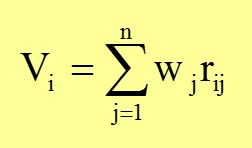
\includegraphics[scale=0.4]{Gambar/saw2.jpg}
	%	\caption{Nilai Preferensi}
	%	\label{fig:nilaipreferensi}
%	\end{figure}
	
	Jika telah melalui proses perhitungan, maka ditemukan sebuah hasil Vi. Nilai Vi yang lebih besar mengindikasikan bahwa alternatif Ai lebih terpilih \cite{karakteristikspk}. Langkah-langkah penyelesain dalam menentukan sebuah keputusan dengan menggunakan metode SAW adalah:
	
	\begin{enumerate}
		\item Menentukan alternatif, yaitu $A_{i}$.
		\item Menentukan kriteria-kriteria yang akan dijadikan acuan dalam mengambil keputusan, yaitu $C_{i}$.
		\item Menentukan nilai rating kecocokan setiap alternatif pada setiap kriteria.
		\item Menentukan bobot preferensi atau tingkat kepentingan (W) setiap kriteria. W = [$W_{1}$ $W_{2}$ $W_{3}$ ... $W_{j}$]
		\item Membuat tabel rating kecocokan dari setiap alternatif pada setiap kriteria.
		\item Membuat matriks keputusan X yang dibentuk dari tabel rating kecocokan dari setiap alternatif pada setiap kriteria. Nilai X setiap alternatif ($A_{i}$) pada setiap kriteria ($C_{j}$) yang sudah ditentukan, dimana i=1,2,3,...,m dan j=1,2,3,...,n.
		 \begin{displaymath} X = 
\left (
\begin{array}{rrrr}
X11 & X12 &... &X1j\\		
. & . & . & .\\
. & . & . & .\\
. & . & . & .\\
			Xi1 & Xi2 &... &Xij\end{array}
\right )	
	\end{displaymath}
	\item Melakukan normalisasi matriks keputusan X dengan cara menghitung nilai rating kinerja ternormalisasi ($r_{ij}$) dari alternatif $A_{i}$ pada kriteria $C_{j}$.
	\item Hasil dari nilai rating kinerja ternormalisasi ($r_{ij}$) membentuk matrik ternormalisasi R.\\
	\begin{displaymath} R = 
\left (
\begin{array}{rrrr}
r11 & r12 &... &r1j\\		
. & . & . & .\\
. & . & . & .\\
. & . & . & .\\
			ri1& ri2&... &rij\end{array}\right )	
	\end{displaymath}
	\item Diperoleh hasil dari penjumlahan perkalian elemen baris matrik ternormalisasi R dengan bobot preferensi W yang bersesuaian dengan elemen kolom matrik W. 
	\item Hasil perhitungan nilai $V_{i}$ yang lebih besar mengindikasikan bahwa alternatif $A_{i}$ merupakan alternatif terbaik sebagai solusi.
	\end{enumerate}
	
	Berdasarkan penjelasan yang telah diberikan sebelumnya, dapat disimpulkan bahwa, metode SAW dapat digunakan dalam kehidupan sehari-hari, termasuk dalam menentukan nama baptis pada agama Katolik. Penentuan nama baptis, tidaklah sembarangan. Dalam menentukannya, terdapat beberapa kriteria.
	
\subsection{Contoh Kasus SAW}
\label{sec:contohsaw}
	
Suatu perusahaan akan memilih seorang karyawan untuk dipromosikan sebagai kepala Cabang \cite{contohsaw}. Perusahaan memberikan 4 kriteria yang digunakan untuk melakukan penilaian terhadap calon karyawan. Kriteria ($C_{i}$) diperlukan oleh perusahaan, agar perusahaan dapat menilai calon karyawan yang dijadikan sebagai kandidat alternatif tersebut. Kriteria ditentukan oleh perusahaan berdasarkan beberapa tes dan praktek. Berikut adalah 4 kriteria yang telah ditentukan oleh perusahaan:
\begin{enumerate}
	\item $C_{1}$ = tes pengetahuan (wawasan)
	\item $C_{2}$ = praktek kepemimpinan
	\item $C_{3}$ = tes kepribadian
	\item $C_{4}$ = tes Inovasi
\end{enumerate}

Pada beberapa kriteria yang sudah ditentukan oleh perusahaan tersebut, akan diberikan bobot pada masing-masing kriteria. Berdasarkan metode SAW, bobot diperlukan dalam sebuah kriteria. Bobot ($W_{j}$) pada masing-masing kriteria ditentukan berdasarkan tingkat kepentingan dari setiap kriteria dan harus berjumlah 1 atau 100\%. Bobot tersebut digunakan untuk menghitung nilai akhir dari alternatif. Perusahaan memberikan bobot untuk setiap kriteria sebagai berikut:
\begin{enumerate}
	\item $C_{1}$ = 35\% = 0.35
	\item $C_{2}$ = 25\% = 0.25
	\item $C_{3}$ = 35\% = 0.35
	\item $C_{4}$ = 5\%  = 0.05
\end{enumerate}

Selain terdapat kriteria, metode SAW juga membutuhkan sebuah alternatif ($A_{i}$). Alternatif pada perusahaan adalah calon karyawan tersebut. Ada 4 calon karyawan yang menjadi kandidat alternatif untuk dipromosikan sebagai kepala cabang. Alternatif diperlukan oleh perusahaan agar perusahaan dapat mengetahui calon karyawan yang tepat untuk dipromosikan sebagai kepala cabang. Terdapat 2 atribut pada metode SAW, yaitu atribut keuntungan (\textit{benefit}) dan biaya (\textit{cost}). Pada kasus ini, alternatif tersebut termasuk dalam atribut keuntungan, karena hasil \textit{output} yang akan dikeluarkan adalah menguntungkan perusahaan. Berikut adalah 4 alternatif yang sudah terdaftar sebagai calon karyawan di perusahaan tersebut:
\begin{enumerate}
	\item $A_{1}$ = Andre,
	\item $A_{2}$ = Aan,
	\item $A_{3}$ = Andi, dan
	\item $A_{4}$ = Arif.
\end{enumerate}

Pada metode SAW membutuhkan sebuah proses normalisasi. Normalisasi adalah sebuah proses yang menormalisasikan matriks keputusan (X) ke suatu skala, yang dapat diperbandingkan dengan semua rating alternatif yang ada. Dengan kata lain, normalisasi adalah proses pengelompokkan data menjadi satu kategori atribut dan diperbandingkan. Pada kasus ini, data dikelompokkan berdasarkan atribut keuntungan (\textit{benefit}). Pada setiap alternatif yang telah dikelompokkan tersebut, diberikan sebuah angka atau nilai. Angka atau nilai tersebut didapatkan dari hasil tes dan praktek pada kriteria yang ditentukan. Berikut adalah tabel nilai alternatif pada setiap kriteria:


\begin{table}[H]
	\centering
	\caption{Tabel Nilai Alternatif}
		\begin{tabular}{|l|r|r|r|r|} \hline
    &
    \multicolumn{4}{|c|}{Kriteria} \\
		\hline
    Alternatif    & $C_{1}$ & $C_{2}$ & $C_{3}$ & $C_{4}$ \\
    \hline
    Andre      & 70&50&80    & 60      \\ \hline
       Aan   &    50&60&82&70      \\ \hline
    Andi       & 85&55&80&75      \\ \hline
    Arif       & 82&75&65&85     \\
    \hline
		
		\end{tabular}
	\label{table:nilaialternatif}
\end{table}


	Dari data yang sudah didapatkan sebelumnya, maka permasalahan pengambilan keputusan suatu perusahaan dapat diselesaikan. Untuk menyelesaikan permasalahan tersebut dibutuhkan penormalisasian. Berikut adalah rumus normalisasi:
	
	\[ r_{ij}  =
  \begin{cases}
    \frac{x_{ij}}{\stackrel{Max}{i} x_{ij}}      & \quad \text{jika } j \text{ adalah atribut keuntungan (\textit{benefit})}\\
	\end{cases}	  
\]
	
	Perhitungan dilakukan untuk masing-masing kriteria pada setiap alternatif. Perhitungan dilakukan dengan cara mengambil $x_{ij}$ pada bagian kolom kriteria $C_{i}$ dan nilai maximum (${\stackrel{Max}{i} x_{ij}}$) dari masing-masing kolom pada setiap kriteria. Sebagai contoh, kriteria 1. Pada kriteria 1, $x_{ij}$ yang akan dihitung pada $r_{11}$ adalah 70, dan kandidat nilai maximumnya (${\stackrel{Max}{i} x_{ij}}$) adalah 70, 50, 85 dan 82. Nilai maximum (${\stackrel{Max}{i} x_{ij}}$) yang didapat adalah 85, sehingga 70 akan dibagi dengan 85. Berikut adalah cara untuk menormalisasikan pada masing-masing kriteria.

	%kolom 1
\begin{enumerate}
	\item Pada $C_{1}$ penyelesaiannya sebagai berikut:
\begin{displaymath}
r_{11} = \frac{70}{max {70;50;85;82}} = \frac{70}{85} = 0.82\\
\end {displaymath}
\begin{displaymath}
r_{21} = \frac{50}{max {70;50;85;82}} = \frac{50}{85} = 0.59\\
\end{displaymath}
\begin{displaymath}
r_{31} = \frac{85}{max {70;50;85;82}} = \frac{85}{85} = 1\\
\end {displaymath}
\begin{displaymath}
r_{41} = \frac{82}{max {70;50;85;82}} = \frac{82}{85} = 0.96\\
\end {displaymath}
%kolom2
\item Pada $C_{2}$ penyelesaiannya sebagai berikut:
\begin{displaymath}
r_{12} = \frac{50}{max {50;60;55;75}} = \frac{50}{75} = 0.67\\
\end{displaymath}
\begin{displaymath}
r_{22} = \frac{60}{max {50;60;55;75}} = \frac{60}{75} = 0.80
\end{displaymath}
\begin{displaymath}
r_{32} = \frac{55}{max {50;60;55;75}} = \frac{55}{75} = 0.73\\
\end{displaymath}
\begin{displaymath}
r_{42} = \frac{75}{max {50;60;55;75}} = \frac{75}{75} = 1
\end{displaymath}
\item Pada $C_{3}$ penyelesaiannya sebagai berikut:
\begin{displaymath}
r_{13} = \frac{80}{max {80;82;80;65}} = \frac{80}{82} = 0.97\\
\end{displaymath}
\begin{displaymath}
r_{23} = \frac{82}{max {80;82;80;65}} = \frac{82}{82} = 1
\end{displaymath}
\begin{displaymath}
r_{33} = \frac{80}{max {80;82;80;65}} = \frac{80}{82} = 0.97\\
\end{displaymath}
\begin{displaymath}
r_{43} = \frac{65}{max {80;82;80;65}} = \frac{65}{82} = 0.79
\end{displaymath}
\item Pada $C_{4}$ penyelesaiannya sebagai berikut:
\begin{displaymath}
r_{14} = \frac{60}{max {60;70;75;85}} = \frac{60}{85} = 0.70\\
\end{displaymath}
\begin{displaymath}
r_{24} = \frac{70}{max {60;70;75;85}} = \frac{70}{85} = 0.82
\end{displaymath}
\begin{displaymath}
r_{34} = \frac{75}{max {60;70;75;85}} = \frac{75}{85} = 0.88\\
\end{displaymath}
\begin{displaymath}
r_{44} = \frac{85}{max {60;70;75;85}} = \frac{85}{85} = 1
\end{displaymath}
\end{enumerate}

Berikut adalah hasil dari nilai rating kinerja yang sudah ternormalisasi:
\begin{displaymath} R = 
\left (
\begin{array}{rrrrrrr}
0.82 & 0.67 & 0.97 & 0.70\\		
0.59 & 0.80 & 1 & 0.82\\
1 & 0 & 0.97 & 0.88 \\
0.96 & 1 & 0.79 & 1 \\
\end{array}\right )	
\end{displaymath}



Proses normalisasi telah selesai dihitung. Dari hasil proses normalisasi didapatkan hasil berupa beberapa data pada masing-masing alternatif terhadap nilai rating kinerja ($r_{ij}$). Pada setiap kriteria terdapat bobot, yaitu W = [$W_{1}$, $W_{2}$, $W_{3}$, $W_{4}$], yang merepresentasikan W = [0.35, 0.25, 0.25, 0.05]. Untuk mendapatkan nilai akhir ($V_{i}$), maka dibutuhkan rumus preferensi, seperti berikut:

\[
 V_{i} =\displaystyle\sum_{j=1}^{n} w_{j} r_{ij}
\]

Perhitungan dilakukan untuk masing-masing alternatif. Sebagai contoh, alternatif 1. Pada alternatif 1, bobot preferensi ($w_{j}$) yang akan dihitung pada nilai akhir ($V_{1}$) adalah 0.35 ($w_{1}$), dan nilai rating kinerja ($r_{ij}$) yang akan dihitung adalah $r_{11}$, $r_{12}$, $r_{13}$, $r_{14}$. Masing-masing $r_{ij}$ pada alternatif 1 akan dikalikan dengan 0.35 dan akan di jumlah. Hasil yang didapat adalah 0.732. Berikut adalah cara untuk mendapatkan nilai akhir pada masing-masing alternatif.

\begin{enumerate}
	\item $V_{1}$ = (0.35)(0.82)+(0.25)(0.67)+(0.25)(0.97)+(0.05)(0.70)= 0.287 + 0.1675 + 0.2425 + 0.035 = 0.732
	\item $V_{2}$ = (0.35)(0.59)+(0.25)(0.80)+(0.25)(1)+(0.05)(0.82)= 0.2065 + 0.2 + 0.25 + 0.041 = 0.6975
	\item $V_{3}$ = (0.35)(1)+(0.25)(0.73)+(0.25)(0.97)+(0.05)(0.88)= 0.35 + 0.1825 + 0.2425 + 0.044 = 0.819
	\item $V_{4}$ = (0.35)(0.96)+(0.25)(1)+(0.25)(0.79)+(0.05)(1)= 0.336 + 0.25 + 0.1975 + 0.05 = 0.8335
\end{enumerate}

Pada nilai akhir ($V_{i}$), nilai yang paling besar dibandingkan nilai yang lain merupakan alternatif terbaik sebagai solusi. Dari hasil perhitungan sebelumnya, didapatkan hasil sebagai berikut:


\begin{table}[H]
	\centering
	\caption{Tabel Nilai Akhir ($V_{i}$)}
		\begin{tabular}{| l | l |} 
     \hline
     & Nilai Akhir ($V_{i}$)  \\ \hline
   $V_{1}$ & 0.732 \\ \hline
   $V_{2}$ & 0.6975   \\ \hline
	 $V_{3}$ & 0.819  \\ \hline
   $V_{4}$ & 0.8335   \\ 
    \hline
		
		\end{tabular}
	\label{table:nilaiakhir1}
\end{table}


Jika hasil perhitungan tersebut diurutkan dari yang paling besar hingga paling kecil, maka $V_{4}$ adalah yang paling besar dan $V_{2}$ adalah yang paling kecil. Berikut adalah hasil yang telah diurutkan secara menurun:

\begin{table}[H]
	\centering
	\caption{Tabel Nilai Akhir ($V_{i}$) Setelah Diurutkan}
		\begin{tabular}{| l | l |} 
     \hline
     & Nilai Akhir ($V_{i}$)  \\ \hline
   $V_{4}$ & 0.8335\\ \hline
	$V_{3}$ & 0.819\\ \hline
	$V_{1}$ & 0.732 \\ \hline
   $V_{2}$ & 0.6975  \\  
    \hline
		
		\end{tabular}
	\label{table:nilaiakhir2}
\end{table}

Dengan demikian, nilai akhir yang paling besar adalah $V_{4}$, sehingga alternatif $A_{4}$ adalah alternatif yang terpilih sebagai alternatif terbaik. Dengan kata lain, Arif akan terpilih sebagai kepala Cabang. Yang dapat dijadikan alternatif lain setelah $A_{4}$ adalah $A_{3}$, $A_{1}$, dan $A_{2}$.


\section{PHP}
\label{sec:php}

PHP adalah bahasa pemrograman \textit{script server-side} yang didesain untuk pengembangan web \cite{php2}.  \textit{Script server-side} adalah bahasa pemrograman web yang pengolahan datanya dilakukan oleh komputer server atau penyedia. Jadi, setiap kali sebuah web dikunjungi oleh komputer server akan mengirimkan data-data yang diminta dari database yang kemudian akan ditampilkan di web. Hal ini berbeda dibandingkan dengan bahasa pemrograman \textit{client-side}, seperti JavaScript yang diproses pada web browser (\textit{client}). Selain itu, PHP juga bisa digunakan sebagai bahasa pemrograman umum. Pada awalnya PHP merupakan kependekan dari \textit{Personal Home Page} (Situs Personal). PHP dikembangkan pada tahun 1995 oleh Rasmus Lerdord dan pada waktu itu PHP masih bernama FI (\textit{Form Interpreted}), dan sekarang dikelola oleh \textit{The} PHP \textit{Group}. Situs resmi PHP beralamat di \url{http://www.php.net}.
	
	Pada awalnya PHP merupakan singkatan dari \textit{Personal Home Page}. Sesuai dengan namanya, PHP digunakan untuk membuat website pribadi. Dalam beberapa tahun, PHP berkembang dan menjelma menjadi bahasa pemrograman web yang \textit{powerful} dan tidak hanya digunakan untuk membuat halaman web sederhana, tetapi juga website populer yang digunakan oleh jutaan orang, seperti wikipedia, wordpress, dan lain-lain.
	
	Saat ini PHP adalah singkatan dari \textit{PHP Hypertext Preprocessor}, sebuah kepanjangan rekursif, yakni permainan kata di mana kepanjangannya terdiri dari singkatan itu sendiri. PHP dapat digunakan dengan gratis dan bersifat \textit{open source} dan PHP dirilis dalam lisensi \textit{PHP License}.
	
	Website dinamis yang bisa dibuat menggunakan PHP adalah situs web yang bisa menyesuaikan tampilan konten tergantung situasi. Website dinamis juga bisa menyimpan data ke dalam database, membuat halaman yang berubah-ubah sesuai \textit{input} dari \textit{user}, memproses \textit{form}, dan lain-lain.
	
	Untuk pembuatan web, kode PHP biasanya di sisipkan ke dalam dokumen HTML. Karena fitur inilah, PHP disebut sebagai \textit{\textbf{Scripting Language}} atau bahasa pemrograman \textbf{\textit{script}}. \textit{\textbf{Scripting language}} merupakan penerjemah yang bertugas untuk menerjemahkan dari bahasa yang ada pada web server. \textit{\textbf{Scripting language}} juga dapat dikatakan salah satu komponen pendukung yang paling penting pada web dan terbagi atas 2 bagian, yaitu \textit{Client Side Scripting} (CSS) dan \textit{Server Side Scripting} (SSS).

\subsection{Kelebihan PHP}
\label{sec:contohphp}

PHP sudah umum digunakan untuk beberapa web. Dengan demikian, PHP sangat bagus mengenai sistem kerjanya. Sehingga PHP memiliki beberapa kelebihan yang lebih baik, dibandingkan bahasa pemrograman lain, yaitu:
\begin{enumerate}
	\item PHP adalah sebuah \textit{\textbf{Scripting language}} yang tidak melakukan sebuah kompilasi atau kerumitan dalam penggunaannya.
	\item Web Server yang mendukung PHP dapat ditemukan di mana-mana dari mulai apache, IIS, Lighttpd, hingga Xitami dengan konfigurasi yang relatif mudah.
	\item Dalam sisi pengembangan lebih mudah.
	\item Dalam sisi pemahaman, PHP adalah\textit{\textbf{Scripting language}} yang paling mudah karena memiliki referensi yang banyak.
	\item PHP adalah bahasa \textit{open source} yang dapat digunakan di berbagai mesin dan dapat dijalankan secara \textit{runtime} melalui console serta juga dapat menjalankan perintah-perintah sistem.
\end{enumerate}
%Tipe data dari PHP ada 8, yaitu:
%\begin{itemize}
%	\item Boolean
%	\item Integer
%	\item Float/Double
%	\item String
%	\item Array
%	\item Object
%	\item Resource
%	\item NULL
%\end{itemize}


\subsection{Contoh Kasus PHP}
\label{sec:contohphp}
	

	Sebagai contoh kasus penggunaan PHP adalah misalkan kita ingin membuat list dari nomor 1 sampai nomor 10. Tetapi umumnya sebelum menyisipkan PHP pada kode HTML, ada beberapa kode dari HTML murni (belum terdapat kode PHP). Berikut adalah contoh kode untuk membuat list dari nomor 1 sampai dengan nomor 10 menggunakan HTML murni.
	
	\begin{lstlisting}
		<!DOCTYPE html>
		<html>
			<head>
				<title>Contoh list dengan HTML</title>
			</head>
			<body>
				<h2>Daftar Absensi Mahasiswa</h2>
						<ol>
							<li>Nama Mahasiswa ke-1</li>
							<li>Nama Mahasiswa ke-2</li>
							<li>Nama Mahasiswa ke-3</li>
							<li>Nama Mahasiswa ke-4</li>
							<li>Nama Mahasiswa ke-5</li>
							<li>Nama Mahasiswa ke-6</li>
							<li>Nama Mahasiswa ke-7</li>
							<li>Nama Mahasiswa ke-8</li>
							<li>Nama Mahasiswa ke-9</li>
							<li>Nama Mahasiswa ke-10</li>							
						</ol>
			</body>
		</html>
	\end{lstlisting}	
	
	%		\begin{figure}[htbp]
	%	\centering
	%		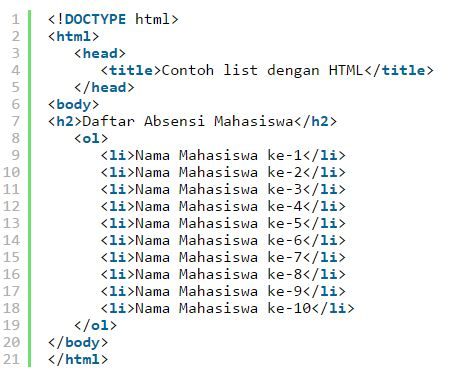
\includegraphics[scale=0.9]{Gambar/php1.JPG}
	%		\caption{Contoh HTML}
	%	\label{fig:php1}
	%\end{figure}
	
	Halaman HTML tersebut dapat dibuat dengan mudah dengan cara melakukan \textit{copy}-\textit{paste} tag\texttt{<li>} sebanyak 10 kali dan mengubah sedikit angka-angka nomor urut di belakangnya. Namun jika yang kita inginkan adalah menambahkan list tersebut menjadi 100 atau 1000 list, cara tersebut menjadi tidak efektif. Jika menggunakan PHP, cara akan menjadi efektif dengan cara membuat perulangan for sebanyak 1000 kali. Berikut adalah contoh kode PHP dengan menggunakan perulangan \texttt{for}.

	\begin{lstlisting}
		<!DOCTYPE html>
		<html>
			<head>
				<title>Contoh list dengan HTML</title>
			</head>
			<body>
				<h2>Daftar Absensi Mahasiswa</h2>
						<ol>
							<?php
									for($i=1;$i<=1000;$i++){
										echo ``<li>Nama Mahasiswa ke-1</li>'';
									}
							?>													
						</ol>
			</body>
		</html>
	\end{lstlisting}	

%\begin{figure}[htbp]
%		\centering
%			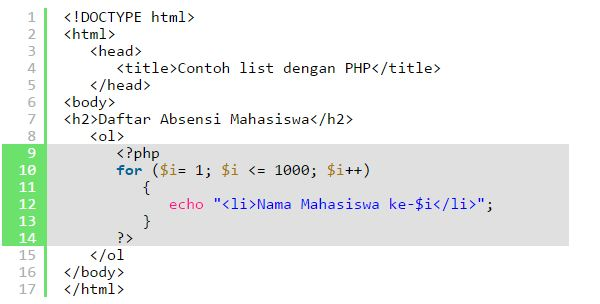
\includegraphics[scale=0.9]{Gambar/php2.JPG}
%			\caption{Contoh PHP}
%		\label{fig:php2}
%	\end{figure}
PHP tidak hanya dapat melakukan pengulangan tersebut, tetapi masih banyak hal 
lain yang bisa dilakukan dengan PHP, seperti menginput data ke database, 
menghasilkan gambar, dan lain sebagainya.

Sama halnya dengan HTML, Java dan kode pemrograman lainnya, PHP juga mempunyai beberapa sintaksis dasar, yaitu:
\begin{itemize}
	\item \texttt{<?php ?>} (Pembatas)
	
	PHP hanya mengeksekusi kode yang ditulis dalam pembatas sebagaimana ditentukan oleh dasar \textit{syntax} PHP. Pembatas yang paling umum adalah ``\texttt{<?php>} '' untuk membuka dan ``\texttt{<?>}'' untuk menutup kode PHP. Tujuan dari pembatas ini adalah untuk memisahkan kode PHP dari kode di luar PHP, seperti HTML, Javascript.	
	\item \texttt{\$} (Variabel)
	
	Variable diawali dengan simbol dolar \texttt{\$}. Contoh variable dapat ditulis sebagai \texttt{\$nama\_variabel}. Penulisan fungsi, penamaan kelas, nama variable adalah ``peka'' akan huruf besar dan huruf kecil. Kedua kutip ganda \texttt{``  ''} dari string memberikan kemampuan untuk interpolasi nilai variabel ke dalam string PHP. PHP menerjemahkan baris sebagai spasi, dan pernyataan harus diakhiri dengan titik koma. %\semicolon.
	
	\item \texttt{/*   */, //, \#} (Komentar)
	
	PHP memiliki 3 jenis \textit{syntax} sebagai komentar pada kode yaitu:
	
	\begin{itemize}
		\item Tanda blok\texttt{ /*   */}, untuk komentar 1 blok
		\item Komentar 2 baris \texttt{//}, untuk komentar 2 baris
		\item Tanda pagar \texttt{\#}, untuk komentar satu baris
	\end{itemize}
	Komentar bertujuan untuk meninggalkan catatan pada kode PHP dan tidak akan diterjemahkan ke program.
	\item \texttt{Fungsi}
	
	Seiring dengan perkembangan PHP, fungsi memiliki berbagai konvensi penamaan. \textit{Syntax} fungsi adalah seperti di bawah ini:
	
	\begin{lstlisting}
		function tampilkan($data=``'')
		{ if ($data) return $data;
				else return 'Tidak ada data';
		}
		
		echo tampilkan (``isi halaman'') //menjalankan fungsi
	\end{lstlisting}
	
	%	\begin{figure}[htbp]
	%	\centering
	%		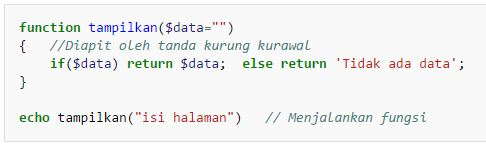
\includegraphics[scale=0.9]{Gambar/php3.JPG}
	%		\caption{Contoh Sintaks Fungsi}
	%	\label{fig:php3}
	%\end{figure}	
\end{itemize}



\section{MySQL}
\label{sec:sql}
MySQL adalah sebuah perangkat lunak sistem manajemen basis data SQL (\textit{Structured Query Language}) atau DBMS (\textit{Database Manajement System}) yang \textit{multithread} dan \textit{multi-user}. \textit{Multithread} adalah sebuah proses dengan \textit{thread} yang banyak dan dapat mengerjakan lebih dari satu tugas dalam satu waktu, sedangkan \textit{multi-user} adalah dapat dijalankan oleh banyak user dalam satu waktu tanpa mengalami kendala. \textit{Thread} adalah unit terkecil dalam suatu proses yang bisa dijadwalkan oleh sistem operasi.  

MySQL merupakan turunan salah satu konsep utama dalam database, yaitu SQL. SQL adalah sebuah konsep pengoperasian database, terutama untuk pemilihan atau seleksi dan pemasukan data, yang memungkinkan pengoperasian data dikerjakan dengan mudah secara otomatis.

\subsection{Kelebihan MySQL}
\label{sec:kelebihansql}

Sebagai database server, MySQL dapat dikatakan lebih unggul dibandingkan database server lainnya dalam \textit{query} data. MySQL memiliki beberapa keistimewaan, antara lain:
		
		\begin{enumerate}
			\item Merupakan salah satu perangkat lunak yang \textit{portable}
			
			Dapat berjalan stabil pada berbagai sistem operasi, seperti Windows, Linux, dan lain sebagainya, sehingga hal ini membuat MySQL menjadi lebih baik dari segi efisiensi dan juga fungsionalitas yang lebih baik. MySQL juga dapat dijalankan untuk mengolah database multi platform. 
			
			\item MySQL merupakan salah satu DBMS yang \textit{open source}
			
			MySQL didistribusikan sebagai perangkat lunak \textit{open source}
			dibawah lisensi GPL, sehingga dapat digunakan secara gratis dan tidak diragukan kualitasnya. 
			
			\item \textit{Multi-user}
			
			Dapat digunakan oleh beberapa pengguna dalam waktu yang bersamaan tanpa mengalami masalah atau konflik, seperti crash dan semacamnya.
			
			\item \textit{Perfomance tuning}
			
			MySQL memiliki kecepatan yang menakjubkan dalam menangani \textit{query} sederhana, dengan kata lain dapat memproses lebih banyak SQL per satuan waktu.
			
			\item Memiliki tipe data yang bervariasi
			
			MySQL memiliki ragam tipe data yang sangat kaya, seperti float, double, char, text, date, dan lain-lain. Dengan beragam tipe data yang didukung oleh MySQL, maka perangkat lunak ini dapat dikategorikan atau digolongkan sebagai salah satu jenis perangkat lunak yang sangat berguna untuk kebutuhan DBMS.
			
			\item Perintah dan fungsi
			
			Memiliki beberapa operator dan fungsi secara penuh yang mendukung perintah \texttt{Select} dan \texttt{Where} dalam perintah (\textit{query}).
			\item Memiliki fitur keamanan yang baik
			
			Memiliki beberapa lapisan keamanan, seperti level subnetmask, nama host, dan izin akses user dengan sistem perizinan yang mendetail serta sandi terenkripsi.
			
			\item Skalabilitas dan Pembatasan
			
			MySQL mampu menangani database dalam skala besar. Selain itu batas indeks yang dapat ditampung mencapai 32 indeks pada tiap tabelnya.
			
			\item Konektivitas
			
			MySQL dapat melakukan koneksi dengan klien menggunakan protokol TCP/IP, UNIX, atau NT.
			
			\item Lokalisasi
			
			MySQL dapat mendeteksi pesan kesalahan pada klien dengan menggunakan lebih dari 20 bahasa. 
			
			\item Antar muka (\textit{interface})
			
			Memiliki antar muka (\textit{interface}) terhadap berbagai aplikasi dan bahasa pemrograman dengan menggunakan fungsi API.
			
			\item Klien dan Peralatan
			
			MySQL dilengkapi dengan berbagai peralatan yang dapat digunakan untuk administrasi basis data, dan pada setiap peralatan yang ada disertakan petunjuk \textit{online}.
			
			\item Struktur Tabel yang fleksibel
			
			MySQL memiliki struktur tabel yang lebih fleksibel dalam menangani \texttt{ALTER TABLE}, dibandingkan basis data lainnya.
			
			\item Dapat diintegrasikan dengan berbagai bahasa pemrograman
			
			MySQL dapat membantu pembangunan sebuah sistem dengan mudah dan juga efektif, karena dapat terintegrasikan dengan berbagai macam bahasa pemrograman standar yang dapat digunakan dalam pembangunan suatu sistem.
			
			\item Tidak membutuhkan spesifikasi perangkat keras yang tinggi
			
			Untuk dapat menjalankan program MySQL ini, maka tidak dibutuhkan spesifikasi minimal komputer yang tinggi, sehingga PC ataupun laptop dapat menggunakan perangkat lunak MySQL dengan baik, tanpa menemui kendala dan masalah mengenai spesifikasinya.
			
			\item RAM kecil dapat menggunakannya.
			
			Jika dibandingkan database lain, MySQL dapat dijalankan pada RAM yang relatif kecil. Hanya dengan memory < 1GB pun dapat menggunakannya.
			\end{enumerate}
			
%\subsection{Contoh Kasus MySQL}
%\label{sec:contohsql}

%Contoh kasus pada penerapan MySQL adalah akan membuat sebuah database dari sebuah toko buku. Toko buku tersebut membutuhkan beberapa tabel untuk menyimpan semua datanya pada MySQL. Aplikasi sederhana ini terdiri dari 3 alur sederhana, yaitu: %Pada aplikasi berikut berisikan daftar buku dan pemprosesan belanja.\\

%\begin{enumerate}
	%\item Daftar buku
	
		%Pada daftar buku menampilkan halaman berisikan sejumlah daftar buku yang diambil dari tabel buku yang tersimpan di database (Gambar \ref{fig:contohsql1}). Pada halaman ini, terdapat daftar buku beserta harganya.
		
		%\begin{figure}[htbp]
		%\centering
			%	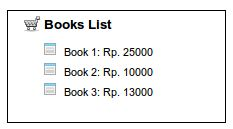
\includegraphics [scale=1]{Gambar/contohsql1.JPG}
			%	\caption{Daftar Buku}
			%\label{fig:contohsql1}
		%\end{figure}
		
%	\item \textit{Form Order}
	
		%Pada \textit{form order} menampilkan form yang berisikan informasi belanja buku dari pengunjung, seperti nama pembeli, alamat, buku yang dibeli, dan jumlahnya yang harus diisi oleh pengunjung, serta terdapat tombol beli agar langsung diarahkan ke halaman proses \textit{order} (Gambar \ref{fig:contohsql2}).
		
			%\begin{figure}[htbp]
	%		\centering
		%		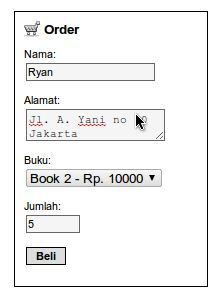
\includegraphics [scale=1]{Gambar/contohsql2.JPG}
				%\caption{\textit{Form Order}}
			%\label{fig:contohsql2}
		%\end{figure}
		
	%\item Proses \textit{Order}
	
	%	Pada proses \textit{Order} memproses informasi dari \textit{form order} yang dimasukkan atau diisi oleh pengunjung (Gambar \ref{fig:contohsql3}). Hasil yang diperoleh adalah berupa halaman konfirmasi, serta memasukkan hasil total pembelian ke dalam tabel.
		
	%		\begin{figure}[htbp]
	%		\centering
	%			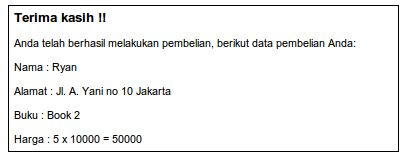
\includegraphics [scale=1]{Gambar/contohsql3.JPG}
	%		\caption{Proses \textit{Order}}
	%	\label{fig:contohsql3}
	%	\end{figure}
%\end{enumerate}

%Untuk menyimpan data atau informasi yang diperlukan oleh aplikasi, perlu disiapkan sebuah database dengan menggunakan phpMyAdmin dengan alamat \url{http://localhost/phpmyadmin} untuk mengatur database, seperti membuat database, membuat tabel dan field, memasukkan data, dan lain sebagainya. Berikut adalah struktur database aplikasi pada Toko Buku Sederhana:
%\begin{itemize}
%	\item \textbf{Nama Database:} bookstore
	
	%	Pada halaman \textit{home} phpMyAdmin klik pada icon ``New'', kemudian akan diarahkan ke tab ``Basis data'' dan masukkan ``bookstore'', sebagai nama databasenya, pada bagian ``Buat basis data'' (Gambar \ref{fig:contohsql6}). Setelah memasukkan ``boostore'', kemudian klik pada tombol ``buat''. Database dengan nama ``boostore'' akan langsung disimpan di MySQL.
		
		%\begin{figure}[htbp]
		%	\centering
		%		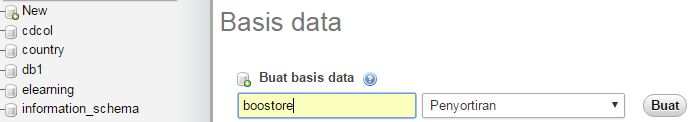
\includegraphics [scale=0.8]{Gambar/contohsql6.JPG}
		%	\caption{Cara membuat database dengan nama ``bookstore''}
		%	\label{fig:contohsql6}
		%\end{figure}

		
	%\item Tabel \textbf{\textit{books:}} berisikan daftar buku (Gambar \ref{fig:contohsql4})
	
	%Pada tabel ini terdapat ID Buku (book\_id), Nama Buku (book\_name), dan Harga Buku (book\_price), tipe, dan juga keterangan.

		%	\begin{figure}[htbp]
		%	\centering
		%		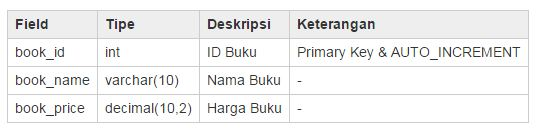
\includegraphics [scale=1]{Gambar/contohsql4.JPG}
		%	\caption{Tabel \textbf{\textit{books}}}
		%	\label{fig:contohsql4}
	%	\end{figure}
		
		
%	Untuk membuat tabel books, caranya adalah pilih database ``boostore'' yang telah dibuat sebelumnya, lalu pada bagian ``Buat Tabel'', terdapat nama yang akan dimasukkan dengan nama ``books'' dan jumlah kolom yang akan diisi 3 kolom. Setelah memasukkan nama dan jumlah kolom, kemudian klik pada tombol ``kirim'' (Gambar \ref{fig:contohsql7}), kemudian akan diarahkan utnuk mengatur struktur tabel.
	
%	\begin{figure}[htbp]
%			\centering
%				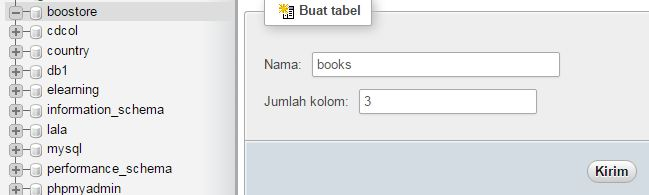
\includegraphics [scale=0.8]{Gambar/contohsql7.JPG}
%			\caption{Cara membuat tabel ``books'' pada database ``bookstore''}
%			\label{fig:contohsql7}
%		\end{figure}
		
%		Setelah mendefinisikan nama tabel, serta banyaknya \textit{field}, langkah selanjutnya adalah mengatur struktur tabel, sehingga menjadi (Gambar \ref{fig:contohsql4}) adalah (Gambar \ref{fig:contohsql8}):
		
		%	\begin{figure}[htbp]
		%	\centering
		%		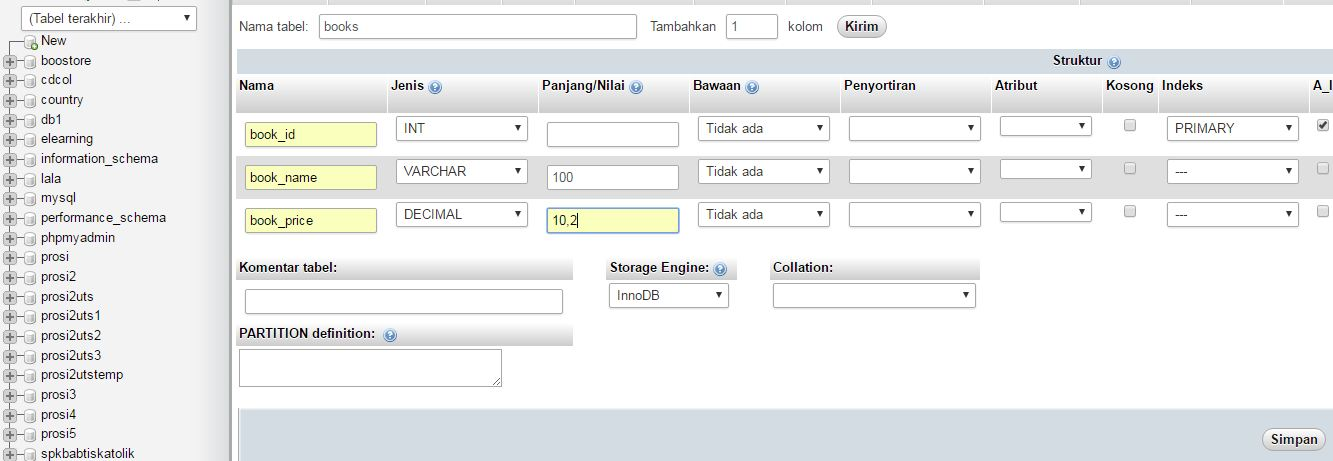
\includegraphics [scale=0.5]{Gambar/contohsql8.JPG}
		%	\caption{Cara mengatur struktur tabel ``books''}
		%	\label{fig:contohsql8}
		%\end{figure}

	%Setelah selesai mengatur struktur tabel tersebut, kemudian klik pada tombol simpan, sehingga akan langsung menyimpan tabel tersebut pada database ``bootstore'' (Gambar \ref{fig:contohsql9}).
	
%		\begin{figure}[htbp]
%			\centering
%				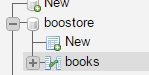
\includegraphics [scale=1]{Gambar/contohsql9.JPG}
%			\caption{Tabel books yang telah tersimpan pada database}
%			\label{fig:contohsql9}
%		\end{figure}
	
	%Kemudian isikan beberapa data contoh pada tabel ``books''. Caranya adalah dengan memilih tabel ``books'', lalu klik tab ``tambahkan'', kemudian masukkan beberapa data di dalamnya, seperti berikut (Gambar \ref{fig:contohsql10}), kemudian klik simpan, akan menjadi seperti (Gambar \ref{fig:contohsql11}):
	
		%\begin{figure}[htbp]
		%	\centering
		%		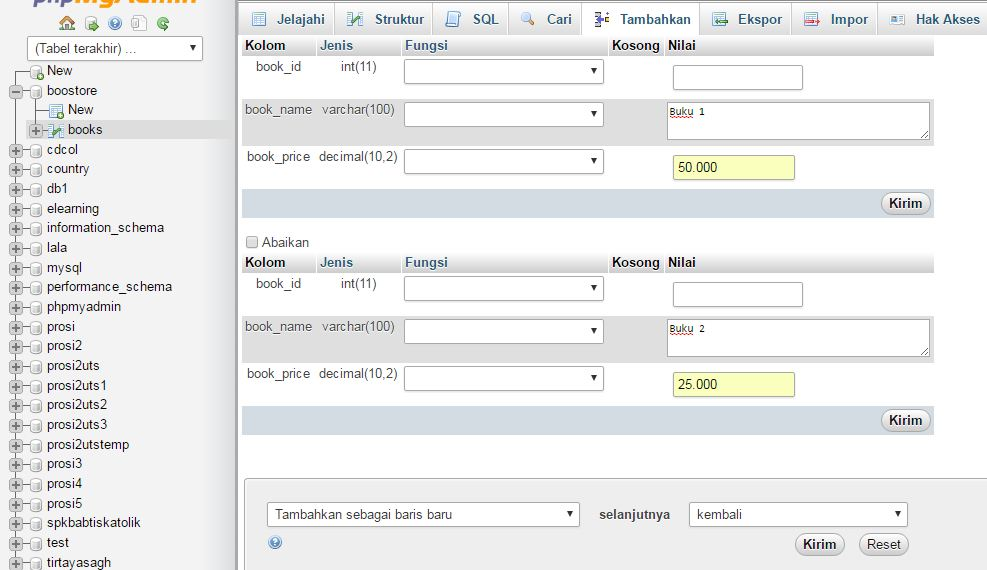
\includegraphics [scale=0.6]{Gambar/contohsql10.JPG}
		%	\caption{Cara memasukkan data buku di tabel ``books''}
		%	\label{fig:contohsql10}
		%\end{figure}
		
		%\begin{figure}[htbp]
			%\centering
			%	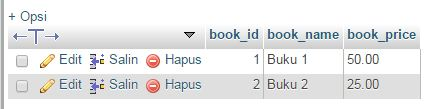
\includegraphics [scale=1]{Gambar/contohsql11.JPG}
			%\caption{Isi Tabel Books}
			%\label{fig:contohsql11}
		%\end{figure}
	
	%\item Tabel \textbf{\textit{orders:}} berisikan order atau pembelian yang dilakukan oleh pengunjung (Gambar \ref{fig:contohsql5})\\
	%Pada tabel ini terdapat ID Order (order\_id), Nama Pembeli (order\_name), Alamat Pembeli (order\_address), ID Buku (book\_id), Jumlah Pembelian (order\_amount), tipe, dan juga keterangan.

		%	\begin{figure}[htbp]
		%	\centering
		%		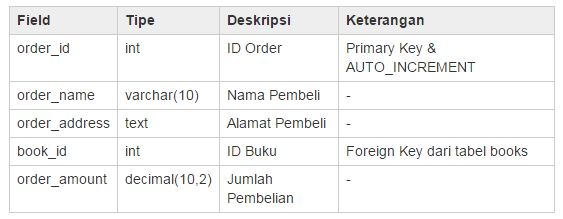
\includegraphics [scale=1]{Gambar/contohsql5.JPG}
		%	\caption{Tabel \textbf{\textit{orders}}}
		%	\label{fig:contohsql5}
		%\end{figure}
		%\end{itemize}
		
		
\subsection{Cara Koneksi MySQL ke PHP}
\label{sec:koneksi}
		
		%cara koneksi mysql ke php
Umumnya tampilan web dapat menampilkan data. Data yang ditampilkan tersebut terdapat pada database. Data yang terdapat pada database akan ditampilkan pada tampilan web, jika terdapat kode koneksi seperti berikut.


	\begin{lstlisting}
		<?php
			$servername = ``localhost'';
			$username = ``root'';
			$password = ``'';
			$dbname = ``boostore'';
			
			//create connection
			$conn=new mysqli($servername, $username, $password, $dbname);
			
			//check connection
			if($conn->connect_error){
				die(``Connection failed: '', $conn->connect_error);
			}
		?>
	\end{lstlisting}	

Keterangan:
\begin{itemize}
	\item	\texttt{\$servername} merupakan tempat database berada. Biasanya yang digunakan adalah localhost.
	\item \texttt{\$username} merupakan nama user yang digunakan, biasanya yang digunakan adalah root. Root merupakan sebuah id database yang terdapat di server.
	\item \texttt{\$password} digunakan untuk masuk ke database.
	\item \texttt{\$dbname} merupakan nama database yang terdapat di \texttt{phpMyAdmin}.
\end{itemize}


		%\begin{figure}[htbp]
		%	\centering
		%		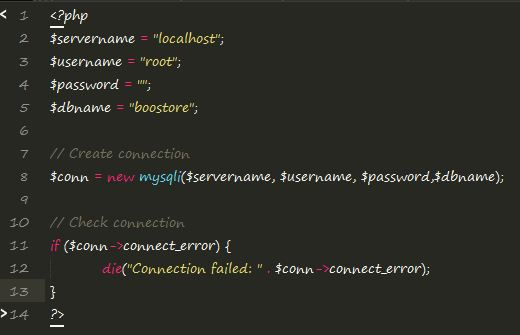
\includegraphics [scale=1]{Gambar/koneksi.JPG}
		%		\caption{Contoh Koneksi}
		%	\label{fig:koneksi}
		%\end{figure}

\section{Bootstrap}
\label{sec:bootstrap}		
		\textit{Boostrap} adalah \textit{front-end framework} yang bagus, dan luar biasa yang mengedepankan tampilan untuk \textit{mobile device}. Bootstrap berguna untuk mempercepat dan mempermudah pengembangan \textit{website} \cite{bootstrap1}. \textit{Bootstrap} menyediakan HTML, CSS, dan JavaScript yang siap pakai dan mudah untuk dikembangkan.
		
		
		\textit{Bootstrap} merupakan \textit{framework} untuk membangun desain web secara responsif. Tampilan web yang dibuat oleh \textit{bootstrap} akan menyesuaikan ukuran layar dari browser yang kita gunakan baik di \textit{desktop}, \textit{tablet}, ataupun \textit{mobile device}. Dengan \textit{bootstrap} kita juga bisa membangun web dinamis ataupun statis.
		
		Dengan demikian, bootstrap sangat dibutuhkan dan sangat membantu bagi para programmer web. Programmer web tidak perlu membuat atau membangun coding baru lagi untuk setiap \textit{device} yang berbeda, karena tampiannya dapat menyesuaikan ukuran layar. 
		%Untuk menggunakan \textit{bootstrap}, harus men-\textit{download resource file} atau file distribusi yang disediakan oleh bootstrap di situs resminya \url{http://getbootstrap.com/}. Pada halaman tersebut terdapat tombol ``Download Bootstrap'' (Gambar \ref{fig:boot1}) klik tombol tersebut, kemudian pilih lagi ``Download Bootstrap'' (Gambar \ref{fig:boot2}). 
		
		%			\begin{figure}[htbp]
			%\centering
				%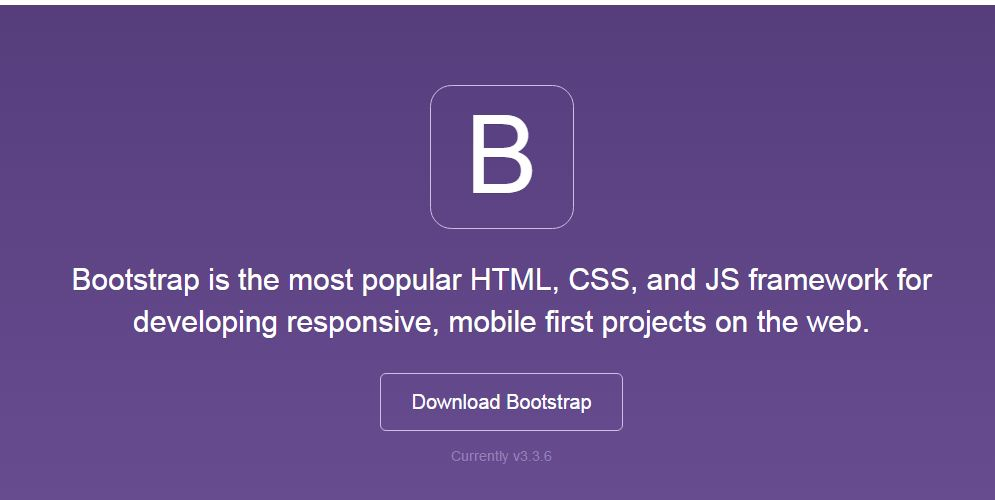
\includegraphics [scale=0.6]{Gambar/boot1.JPG}
		%	\caption{Tampilan Bootstrap}
			%\label{fig:boot1}
		%\end{figure}
		
		%\begin{figure}[htbp]
			%\centering
				%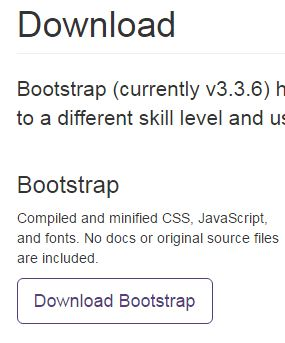
\includegraphics [scale=0.8]{Gambar/boot2.JPG}
			%\caption{Tampilan Bootstrap}
			%\label{fig:boot2}
	%	\end{figure}
		
		
			%Setelah di-\textit{download}, kemudian \textit{extract download}-an tersebut dan dapat langsung digunakan.\\
			
			
		%	Kelebihan dari bootstrap adalah \cite{bootstrap2}:
			
			%\begin{itemize}
				%\item Kompatibel di semua browser
				%\item \textit{Open source}
				%\item Bootstrap lebih lengkap karena mencakup HTML, CSS, dan JavaScript, yang juga mendukung responsif web desain.
				%\item Bootstrap membagi lebar layar menjadi 12 bagian, sehingga pembagian kolom per kolom tampilan web akan menjadi lebih mudah.
			%\end{itemize}


%			Fitur-fitur yang dimiliki bootstrap adalah sebagai berikut:
			
	%		\begin{itemize}
		%		\item Grid System\\
			%	Default 12 kolom
				%\item Layout\\
				%Fixed, Fluid, Responsive
				%\item Fundamental HTML Element Styles\\
				%Typography, tables, forms, buttons, icons, images
				%\item Components\\
				%Dropdown, navigation, buttons groups, breadcrumb, pagination, label, thumbnail, alert message, dan lain sebagainya
				%\item JavaScript\\
				%Dropdown, alert, carousel, dan lain sebagainya.
			%\end{itemize}
		%Terdapat beberapa metode dalam SPK, salah satunya adalah SAW (\textit{Simple Additive Weighting}). Metode ini juga sering disebut dengan metode penjumlahan berbobot. Konsep dasar metode SAW adalah mencari penjumlahan terbobot dari rating kinerja pada setiap alternatif pada semua atribut. Metode SAW membutuhkan proses normalisasi matriks keputusan ke suatu skala yang dapat diperbandingkan dengan semua rating alternatif yang ada.